% =============================================================
% main.tex  --  Disease-Diagnosis-RAG-System (Bao cao Phase 1)
% Bibliography: dung FILE references.bib
% KHONG dat \begin{filecontents*}[overwrite]{references.bib} o day,
% neu khong file references.bib that se bi ghi de -> cite undefined.
% Yeu cau: references.bib phai nam cung thu muc voi main.tex khi build.
% =============================================================
\documentclass[12pt]{ai_conquer2026}
\addbibresource{references.bib}

% ---- Bo sung goi & sua tran le (khong dung vao file .cls goc) ----
\usepackage{tikz}
\usetikzlibrary{arrows.meta,positioning,calc}
\usepackage{pgfplots}
\pgfplotsset{compat=1.16}
% Breakable inline file paths/code (url pkg comes from hyperref; avoids clash with TikZ \path)
\DeclareUrlCommand\code{\urlstyle{tt}}
\titleformat{\section}{\normalfont\huge\bfseries\raggedright}{\thesection}{0.6em}{}
\titleformat{\subsection}{\normalfont\Large\bfseries\raggedright}{\thesubsection}{0.6em}{}
\setlength{\emergencystretch}{3em}
\tikzset{
  stage/.style={rectangle, rounded corners, draw=aivnGreen, thick, fill=aivnGreen!10, align=center, minimum height=1.0cm, inner sep=4pt, font=\small},
  future/.style={rectangle, rounded corners, draw=gray!70, thick, dashed, fill=gray!12, align=center, minimum height=1.0cm, inner sep=4pt, font=\small},
  flow/.style={-{Latex[length=2.4mm]}, thick, draw=aivnGreen!85},
  twoway/.style={{Latex[length=2.4mm]}-{Latex[length=2.4mm]}, thick, draw=aivnGreen!85}
}

\title{%
  \begin{center}
        \IfFileExists{Figures/group\_logo.png}{\includegraphics[width=2.8cm]{Figures/group\_logo.png}\\[1ex]}{}
        \Large {AI VIET NAM -- AI Conquer 2026}\\[.5ex]
        \Huge \textbf{Hệ thống Hỏi--Đáp Hỗ trợ Chẩn đoán Bệnh dựa trên RAG trên bộ dữ liệu DDXPlus}\\[.8ex]
        \large \textnormal{\textit{A Retrieval-Augmented Generation System for Disease Diagnosis Support on the DDXPlus Dataset}}\\[.5ex]
  \end{center}
}

% Author --------------------------------------------------------------------
\posttitle{
\author{
\begin{minipage}{\textwidth}
\centering
\textbf{Nhóm Med\_Pharm\_Bio\_Nexus}\\[0.8em]
\begin{tabular}{lll}
\textbf{Họ và tên} & \textbf{Vị trí} & \textbf{Vai trò}\\[0.3em]
Nguyễn Minh Tú & AI Engineer (Pipeline) & Thành viên\\
Nguyễn Thị Diễm Hương & QA / Reviewer & Thành viên\\
Hoàng Phước Nguyên & AI Engineer (Data) & Thành viên\\
Vương Đình Minh Trí & Tech Leader & Thành viên\\
Nguyễn Văn Thương & AI Engineer (Model) & Quản lý nhóm\\
\end{tabular}
\end{minipage}
}
}
\date{}

% Header --------------------------------------------------------------------
\pagestyle{fancy}
\fancyhf{}
\lhead{\href{https://www.facebook.com/aivietnam.edu.vn}{\textcolor{aivnGreen}{\bfseries AI VIET NAM (AI Conquer 2026)}}}
\rhead{\href{https://aivietnam.edu.vn/}{\textcolor{aivnGreen}{\bfseries aivietnam.edu.vn}}}
\fancyfoot[C]{\thepage}
\renewcommand{\headrulewidth}{1.0pt}
\renewcommand{\headrule}{{\color{aivnGreen}\hrule width\headwidth height\headrulewidth \vskip-\headrulewidth}}

\begin{document}
\maketitle
\vspace{-1.5em}
\setlength{\epigraphwidth}{0.6\textwidth}
\section{Tóm tắt nghiên cứu}
% [NHÁP -- Phụ trách: Nguyễn Văn Thương. Nhóm rà soát & xác nhận trước khi nộp.]

Chẩn đoán bệnh dựa trên triệu chứng là một bài toán cốt lõi trong lĩnh vực \textbf{Healthcare AI}, nơi việc truy xuất đúng tri thức y khoa có vai trò quyết định đến độ tin cậy và an toàn của hệ thống hỗ trợ ra quyết định lâm sàng. Nghiên cứu này xây dựng và đánh giá một hệ thống \textbf{Retrieval-Augmented Generation (RAG)} hỗ trợ chẩn đoán bệnh, sử dụng bộ dữ liệu công khai \textbf{DDXPlus}~\cite{ddxplus2022} gồm \textbf{49 bệnh} và \textbf{223 bằng chứng triệu chứng (evidences)}. Nhóm làm việc trên \textbf{DDXPlus (English) phiên bản 2, đăng ngày 10/03/2026} trên Figshare.

Chúng tôi xây dựng một Knowledge Base (KB) mô tả bệnh từ DDXPlus, chuẩn hoá và kiểm định chất lượng KB, sau đó so sánh ba chiến lược truy xuất: \textbf{BM25} (lexical), \textbf{Dense} (mô hình \texttt{BAAI/bge-small-en-v1.5}, 384 chiều, độ đo cosine) và \textbf{Hybrid} (hợp nhất thứ hạng bằng Reciprocal Rank Fusion, RRF $k=60$).

\textbf{Lưu ý về phương pháp đo:} các con số EXP-01/EXP-02 trong báo cáo này là kết quả của một \textbf{harness Python thuần, brute-force in-memory} trên 49 tài liệu KB, chạy độc lập với hạ tầng tìm kiếm. Đây là \textit{mốc tham chiếu / trần trên} cho chất lượng logic truy xuất trên cùng KB và normalizer. Số liệu \textit{production} được đo trên \textbf{pipeline OpenSearch thật}: lần chạy đầy đủ ngày \textbf{26/06/2026} trên \textbf{toàn bộ $n=132{,}448$ ca} (thay cho lần chạy thử trên mẫu trước đó) cho kết quả nhất quán với offline -- riêng BM25 tái lập gần như khít (Hit@1 98.65\% production vs 98.47\% offline) -- xác nhận độ tin cậy của cả harness lẫn hạ tầng (xem mục Kết quả và Thảo luận).

Kết quả chính theo Hit@1 (Python thuần, $n=132{,}448$): BM25 + \textit{description} đạt \textbf{98.78\%} (MRR 0.9937); Hybrid-RRF + \textit{description} đạt \textbf{91.95\%} (MRR 0.9570); Dense + \textit{description} đạt \textbf{84.28\%} (MRR 0.9027). Hai phát hiện đáng chú ý: (i) trường \textit{description} cải thiện đều cả ba phương pháp; (ii) thiết kế đánh giá hiện tại thiên về \textit{lexical} (truy vấn là token đã chuẩn hoá, trùng khớp từ vựng với KB), nên lợi thế ngữ nghĩa của dense/hybrid chưa được phản ánh đầy đủ.

\textbf{Đóng góp chính:} (1) xây dựng và kiểm định KB DDXPlus (chuẩn hoá evidence, rà soát ánh xạ mã ICD-10); (2) thiết lập khung đánh giá truy xuất theo Hit@1/3/5, MRR và NDCG@5, kèm quy trình đối chiếu \textbf{Python thuần với OpenSearch trên toàn tập}; (3) so sánh hệ thống truy xuất lexical/dense/hybrid trên quy mô đầy đủ và phân tích trung thực giới hạn của bài đánh giá.
\newpage
\setcounter{tocdepth}{2}
\tableofcontents
\thispagestyle{fancy}
\newpage
\section{Giới thiệu (Introduction)}
% [NHÁP -- Phụ trách: Nguyễn Văn Thương.]

Đề tài thuộc lĩnh vực giao thoa giữa \textbf{Healthcare AI} và \textbf{Xử lý ngôn ngữ tự nhiên (NLP)}, cụ thể là bài toán \textbf{truy xuất tri thức phục vụ hỗ trợ chẩn đoán bệnh} theo khung Retrieval-Augmented Generation (RAG).

Trong thực hành lâm sàng, một bệnh nhân thường được mô tả bằng một tập hợp triệu chứng và tiền sử (evidences). Hệ thống cần truy xuất đúng các bệnh lý liên quan từ một kho tri thức y khoa để hỗ trợ bác sĩ thu hẹp chẩn đoán phân biệt. Bài toán này quan trọng vì: (i) sai sót trong truy xuất tri thức có thể dẫn tới gợi ý chẩn đoán sai lệch; (ii) hệ thống RAG cho phép kiểm soát nguồn tri thức và giảm hiện tượng ảo giác (hallucination) của mô hình ngôn ngữ lớn.

\textbf{Khó khăn hiện tại:} dữ liệu y khoa có độ chồng lấp triệu chứng cao giữa các bệnh; truy vấn thực tế thường diễn đạt tự nhiên, thiếu hoặc nhiễu thông tin; và các mô hình embedding phổ thông chưa được tối ưu cho miền y khoa.

\textbf{Mục tiêu nghiên cứu:} xây dựng một baseline RAG rõ ràng trên DDXPlus, thiết lập một bộ số liệu nền bằng Python thuần để kiểm soát logic truy xuất, rồi đối chiếu với pipeline OpenSearch thật trước khi mở rộng sang sinh câu trả lời.

Các đóng góp chính của nghiên cứu:
\begin{itemize}
\item Xây dựng và kiểm định Knowledge Base bệnh học từ DDXPlus (49 bệnh, 223 evidences), gồm chuẩn hoá evidence và rà soát ánh xạ mã ICD-10.
\item Thiết lập khung đánh giá truy xuất chuẩn (Hit@1/3/5, MRR@5, NDCG@5) trên toàn bộ tập validate ($n=132{,}448$).
\item So sánh ba chiến lược truy xuất BM25, Dense (BGE-small-en-v1.5) và Hybrid (RRF), kèm ablation về vai trò của trường \textit{description}.
\item Thiết kế quy trình đối chiếu \textbf{Python thuần với OpenSearch} để bảo đảm số liệu production đáng tin cậy, và phân tích trung thực giới hạn của thiết kế đánh giá.
\end{itemize}
% =============================================================
% sec03_baitoan.tex  --  Muc III: Bai toan nghien cuu (Research Problem)
% Bao cao Phase 1 -- Disease-Diagnosis-RAG-System
% Trich dan: IEEE numeric (biblatex, style=ieee) qua \cite{...}
% Cac khoa trich dan su dung: jarvelin2002ndcg
% Luu y: khoa tren phai co trong references.bib truoc khi build.
% Luu y noi dung: gia thuyet phat bieu co dieu kien; re-ranking thuoc Phase 2, khong kiem chung o Phase 1.
% =============================================================

\section{Bài toán nghiên cứu (Research Problem)}
\label{sec:baitoan}

\begin{itemize}
    \item \textbf{Tên bài toán:} Truy xuất tri thức y khoa (information retrieval) phục vụ hỗ trợ chẩn đoán bệnh trong khung RAG.
    \item \textbf{Input:} Một truy vấn biểu diễn tập bằng chứng và triệu chứng (evidences) của bệnh nhân, đã được chuẩn hoá theo cùng quy ước với KB.
    \item \textbf{Output:} Danh sách bệnh (tài liệu KB) được xếp hạng theo độ liên quan; lấy top-$K$ để hỗ trợ chẩn đoán phân biệt.
    \item \textbf{Mục tiêu nghiên cứu:} Tối đa hoá độ chính xác truy xuất ở vị trí đầu (Hit@1), đồng thời giữ chất lượng xếp hạng tổng thể (MRR, NDCG@5) cao.
    \item \textbf{Metric đánh giá:} Hit@1, Hit@3, Hit@5, MRR, NDCG@5~\cite{jarvelin2002ndcg}.
\end{itemize}

\textbf{Giả thuyết nghiên cứu:} Giả thuyết được phát biểu theo hướng có điều kiện, gắn liền với đặc điểm của truy vấn đầu vào:
\begin{itemize}
    \item \textit{Với truy vấn đã được token hoá (trùng khớp từ vựng cao với KB):} Chúng tôi kỳ vọng BM25 đạt hiệu quả rất cạnh tranh nhờ tín hiệu khớp từ khoá mạnh.
    \item \textit{Với truy vấn diễn đạt tự nhiên (thiếu hoặc nhiễu thông tin):} Thành phần Dense (embedding ngữ nghĩa) và cơ chế Hybrid hợp nhất thứ hạng bằng RRF được kỳ vọng sẽ bổ khuyết cho BM25, nhờ khả năng nắm bắt tương đồng ngữ nghĩa vượt ra ngoài mức trùng khớp bề mặt.
\end{itemize}

Nói cách khác, đóng góp của Dense và Hybrid phụ thuộc vào mức độ tự nhiên của truy vấn, và chỉ bộc lộ đầy đủ khi thiết kế đánh giá phản ánh được dạng truy vấn thực tế. Giả thuyết này cần được kiểm chứng bằng một bộ đánh giá sát thực tế hơn, và được bàn cụ thể ở mục Thảo luận và Hạn chế.

Trong phạm vi Phase~1, Hybrid được hiện thực bằng hợp nhất thứ hạng RRF giữa BM25 và Dense; thành phần re-ranking chuyên biệt, ví dụ một mô hình cross-encoder, chưa được đưa vào và được dành cho Phase~2. Vì vậy, các kỳ vọng liên quan đến re-ranking chỉ mang tính định hướng cho giai đoạn sau, không nằm trong phạm vi kiểm chứng của báo cáo này.
% =============================================================
% sec04_relatedwork.tex  --  Muc IV: Tong quan nghien cuu lien quan (Related Work)
% Bao cao Phase 1 -- Disease-Diagnosis-RAG-System
% Trich dan: IEEE numeric (biblatex, style=ieee) qua \cite{...}
% Cac khoa trich dan su dung: lewis2020rag, ji2023hallucination, robertson2009bm25,
%   karpukhin2020dpr, reimers2019sbert, xiao2024cpack, cormack2009rrf, nogueira2019bert,
%   ddxplus2022, xiong2024mirage
% Luu y: 10 khoa tren phai co trong references.bib truoc khi build.
% =============================================================

\section{Tổng quan nghiên cứu liên quan (Related Work)}
\label{sec:relatedwork}

Khung retrieval-augmented generation (RAG) do Lewis và cộng sự đề xuất~\cite{lewis2020rag} kết hợp truy xuất tri thức phi tham số với sinh văn bản cho các tác vụ đòi hỏi nhiều tri thức, cho phép cập nhật nguồn tri thức và giảm hiện tượng ảo giác của mô hình ngôn ngữ lớn~\cite{ji2023hallucination}. Đây là khung nền cho hệ thống của chúng tôi; trong phạm vi Phase~1, nhóm tập trung hoàn thiện và đánh giá thành phần truy xuất, vốn quyết định chất lượng đầu vào cho bước sinh câu trả lời ở giai đoạn sau.

Ở hướng truy xuất lexical, BM25 trong khung probabilistic relevance~\cite{robertson2009bm25} là một baseline mạnh, khớp từ vựng chính xác nhưng dễ bỏ sót khi truy vấn và tài liệu diễn đạt khác nhau về mặt ngữ nghĩa. Đặc điểm này phù hợp với dữ liệu evidence đã được chuẩn hoá của chúng tôi, nơi truy vấn và KB dùng chung một quy ước biểu diễn.

Ở hướng truy xuất Dense, các mô hình embedding như DPR~\cite{karpukhin2020dpr} và Sentence-BERT~\cite{reimers2019sbert} biểu diễn truy vấn và tài liệu trong cùng một không gian vector để khớp theo ngữ nghĩa, với chất lượng phụ thuộc nhiều vào dữ liệu huấn luyện và miền ứng dụng. Trong nghiên cứu này, nhóm sử dụng họ embedding BGE~\cite{xiao2024cpack} (bge-small-en-v1.5) làm đại diện cho hướng Dense.

Để dung hoà hai hướng trên, các phương pháp Hybrid hợp nhất kết quả từ nhiều hệ truy xuất. Reciprocal rank fusion (RRF)~\cite{cormack2009rrf} hợp nhất thứ hạng mà không cần huấn luyện thêm, cân bằng thế mạnh khớp từ vựng của lexical và khớp ngữ nghĩa của Dense; đây chính là cơ sở cho biến thể Hybrid của chúng tôi.

Một hướng bổ sung là re-ranking, trong đó cross-encoder trên nền BERT~\cite{nogueira2019bert} tinh chỉnh lại top-$K$ với độ chính xác cao hơn nhưng chi phí tính toán lớn hơn. Vì phạm vi và tài nguyên của giai đoạn hiện tại, nhóm xếp thành phần này vào Phase~2 và không đưa vào đánh giá của báo cáo này.

Trong lĩnh vực y khoa, bộ dữ liệu DDXPlus~\cite{ddxplus2022} có mức độ chồng lấp triệu chứng cao giữa các bệnh và yêu cầu khả năng kiểm chứng nguồn tri thức, khiến bài toán truy xuất trở nên nhạy cảm với cả chất lượng KB lẫn cách biểu diễn truy vấn. Gần đây, các nỗ lực chuẩn hoá đánh giá RAG cho y khoa như MIRAGE~\cite{xiong2024mirage} đã cung cấp benchmark cho tác vụ hỏi đáp y khoa; tuy nhiên, các benchmark này tập trung vào chất lượng câu trả lời sinh ra hơn là so sánh trực tiếp các chiến lược truy xuất.

Để làm rõ bối cảnh hiệu năng trên DDXPlus: Bảng~\ref{tab:baseline_ddxplus} tóm tắt các kết quả từ công trình gốc của Fansi Tchango và cộng sự~\cite{ddxplus2022}. Các tác giả đã đánh giá mức độ chính xác trên hai hệ thống AARLC và BASD. Điểm chung của các phương pháp này là đều tiếp cận theo hướng hội thoại đầu cuối (end-to-end), tối ưu hóa luồng tương tác nhiều lượt với bệnh nhân thay vì bóc tách riêng lẻ năng lực của hệ truy xuất tĩnh. Số liệu cũng minh chứng rõ: khi mô hình được huấn luyện để sinh ra một danh sách chẩn đoán phân biệt thay vì chỉ dự đoán một bệnh duy nhất, việc đánh giá bắt buộc phải xem xét toàn bộ danh sách (đại diện qua chỉ số GTPA) thay vì chỉ nhìn vào vị trí top-1.

\begin{table}[H]
    \centering
    \begin{threeparttable}
        \caption{Tổng hợp hiệu năng của các hệ thống chẩn đoán baseline trên bộ dữ liệu DDXPlus~\cite{ddxplus2022}.}
        \label{tab:baseline_ddxplus}
        \small
        \begin{tabular}{lccc}
            \toprule
            \textbf{Phương pháp (Baseline)}              & \textbf{GTPA@1} & \textbf{GTPA} & \textbf{Hướng tiếp cận} \\
            \midrule
            AARLC (Diff $\times$)~\cite{ddxplus2022}     & 99.21\%         & 99.97\%       & Hội thoại đầu cuối      \\
            BASD (Diff $\times$)~\cite{ddxplus2022}      & 97.15\%         & 98.82\%       & Hội thoại đầu cuối      \\
            AARLC (Diff $\checkmark$)~\cite{ddxplus2022} & 75.39\%         & 99.92\%       & Hội thoại đầu cuối      \\
            BASD (Diff $\checkmark$)~\cite{ddxplus2022}  & 67.71\%         & 99.30\%       & Hội thoại đầu cuối      \\
            \bottomrule
        \end{tabular}
        \begin{tablenotes}[flushleft]
            \footnotesize
            \item \textit{Ghi chú:} Diff ($\checkmark/\times$) cho biết mô hình có được huấn luyện để dự đoán chẩn đoán phân biệt (differential diagnosis) hay không. Theo nguyên bản của Fansi Tchango và cộng sự~\cite{ddxplus2022}, GTPA@1 chỉ phù hợp để đánh giá mô hình được huấn luyện dự đoán bệnh gốc (Diff $\times$). Ngược lại, đối với mô hình dự đoán differential (Diff $\checkmark$), việc bệnh gốc không nằm ở vị trí đầu tiên là bản chất của thuật toán, do đó chỉ số đánh giá tổng thể phù hợp là GTPA. Số liệu trích xuất từ Table~3 của~\cite{ddxplus2022}.
        \end{tablenotes}
    \end{threeparttable}
\end{table}

\textbf{Khoảng trống nghiên cứu.} Phần lớn công trình nêu trên đánh giá truy xuất trên miền mở (open-domain QA) hoặc đề xuất từng phương pháp riêng lẻ cho bài toán hội thoại đầu cuối, còn các benchmark y khoa hiện có thì đang nghiêng về hỏi đáp. Theo hiểu biết của chúng tôi, hiện chưa có benchmark chuẩn hóa nào đánh giá đồng thời ba chiến lược truy xuất tĩnh (lexical, dense và hybrid) trên cùng một knowledge base DDXPlus. Bên cạnh đó, ảnh hưởng của lựa chọn chỉ số đánh giá và quy trình truy xuất đối với kết luận về hiệu quả của từng phương pháp vẫn chưa được phân tích một cách hệ thống. Nghiên cứu này nhằm bước đầu lấp đầy khoảng trống đó bằng cách xây dựng một khung đánh giá minh bạch và độc lập cho khâu truy xuất trước khi tiến tới xây dựng hệ thống hỏi đáp hoàn chỉnh.

% =============================================================
% sec05_phuongphap.tex  --  Muc V: Phuong phap nghien cuu (Methodology)
% Bao cao Phase 1 -- Disease-Diagnosis-RAG-System
% Trich dan: who2019icd10, xiao2024cpack, malkov2018hnsw, qwen2025qwen3
% =============================================================

\section{Phương pháp nghiên cứu (Methodology)}
\label{sec:phuongphap}

\subsection{Tổng quan pipeline hai tầng (Two-Layer RAG)}

Thiết kế A (DDXPlus-only, \textit{retrieval-first}) bao gồm năm giai đoạn. Đầu tiên, \textbf{Knowledge Base (KB)} được xây dựng từ định nghĩa bệnh và các bằng chứng (evidence) sau khi được tiền xử lý và chuẩn hoá bằng các kỹ thuật NLP. Tiếp theo, KB được \textbf{lập chỉ mục} trên OpenSearch với hai loại chỉ mục: chỉ mục từ vựng phục vụ BM25 và chỉ mục vector phục vụ truy xuất k-NN.

Ở giai đoạn \textbf{truy xuất}, hệ thống hỗ trợ ba chiến lược: BM25 (lexical retrieval), Dense Retrieval (semantic retrieval dựa trên embedding và độ tương đồng cosine) và Hybrid Retrieval, trong đó kết quả của BM25 và Dense được hợp nhất bằng kỹ thuật Reciprocal Rank Fusion (RRF). Các tài liệu top-$K$ sau truy xuất được đưa qua bước \textbf{re-ranking} bằng cross-encoder nhằm cải thiện chất lượng xếp hạng. Thành phần này đã được hiện thực trong Phase~1 nhưng chỉ được đánh giá định lượng ở Phase~2. Cuối cùng, các tài liệu đã được xếp hạng sẽ được sử dụng làm ngữ cảnh để \textbf{sinh câu trả lời} bằng LLM trong Phase~2.

Để tách biệt chất lượng của thuật toán truy xuất khỏi ảnh hưởng của hạ tầng triển khai, mỗi chiến lược được đánh giá trên hai môi trường thực thi song song: (i) chế độ \textit{offline} (in-memory, bằng Python thuần) làm mốc tham chiếu và (ii) hệ thống OpenSearch, sử dụng các cơ chế lập chỉ mục và truy xuất tương ứng trong môi trường triển khai thực tế.

\begin{figure}[H]
    \centering
    \resizebox{\textwidth}{!}{%
        \begin{tikzpicture}[node distance=0.9cm]
            \node[stage, text width=2.1cm] (q) {Truy vấn bệnh nhân\\(EVIDENCES + tuổi/giới)};
            \node[stage, text width=2.0cm, right=of q] (pre) {Tiền xử lý\\decode + chuẩn hoá};
            \node[stage, text width=2.5cm, right=of pre] (hyb) {Truy xuất Hybrid\\BM25 (keyword\_text) + k-NN (BGE 384-d)};
            \node[stage, text width=1.9cm, right=of hyb] (rrf) {RRF $k=60$\\$\rightarrow$ top-20};
            \node[future, text width=1.9cm, right=of rrf] (rr) {Re-ranking\\top-20 $\rightarrow$ top-5\\(Phase 2)};
            \node[future, text width=1.9cm, right=of rr] (gen) {Sinh câu trả lời\\Qwen3-8B\\(Phase 2)};
            \draw[flow] (q) -- (pre);
            \draw[flow] (pre) -- (hyb);
            \draw[flow] (hyb) -- (rrf);
            \draw[flow] (rrf) -- (rr);
            \draw[flow] (rr) -- (gen);
        \end{tikzpicture}}
    \caption{Pipeline RAG hai tầng (Thiết kế A). Khối nét liền: hoàn thiện và đánh giá ở Phase 1. Khối nét đứt: re-ranking (mã nguồn hoàn thiện ở cuối Phase 1, đánh giá định lượng ở Phase 2) và sinh câu trả lời (Phase 2).}
    \label{fig:pipeline}
\end{figure}

\subsection{Từ dữ liệu thô đến Knowledge Base: quy trình NLP}

Knowledge Base (KB) được xây dựng thông qua kịch bản \texttt{scripts/build\_kb.py}, đảm nhiệm vai trò chuyển đổi dữ liệu thô thành phiên bản chuẩn hoá phục vụ cho khâu truy xuất. Toàn bộ quá trình chuẩn hoá sử dụng chung mô-đun tiền xử lý \texttt{src/services/rag/preprocess.py} cho cả hai giai đoạn: xây dựng chỉ mục (ingest) và xử lý truy vấn (query), qua đó bảo đảm văn bản được chuẩn hoá nhất quán giữa thời điểm lập chỉ mục và thời điểm truy xuất.

\paragraph{(a) Nguồn dữ liệu và trích xuất trường.}
Knowledge Base được xây dựng từ hai tệp của bộ dữ liệu DDXPlus: \texttt{release\_conditions.json} (49 bệnh) và \texttt{release\_evidences.json} (223 evidence). Đối với mỗi bệnh, hệ thống trích xuất các trường cốt lõi gồm tên bệnh (\texttt{cond-name-eng}), danh sách evidence trong \texttt{symptoms} và \texttt{antecedents}, mức độ nghiêm trọng (\texttt{severity}, trên thang điểm từ 1 đến 5) và mã ICD-10 (\texttt{icd10-id}).

\paragraph{(b) Chuẩn hoá cụm triệu chứng (\texttt{normalize\_symptom\_phrase}).}
Mỗi mã evidence được ánh xạ sang câu hỏi tiếng Anh (\texttt{question\_en}) rồi chuyển đổi thành một cụm danh từ biểu diễn triệu chứng thông qua hàm \texttt{normalize\_symptom\_phrase}. Quy trình chuẩn hoá bao gồm các bước sau:
\begin{enumerate}[leftmargin=1.4em,itemsep=2pt]
    \item Áp dụng \textbf{bảng ghi đè (override table)} cho các câu hỏi đặc biệt không thể xử lý chính xác bằng các quy tắc tổng quát. Bảng này gồm 24 phép ánh xạ được xây dựng thủ công nhằm bảo toàn ý nghĩa lâm sàng. Ví dụ, \textit{``Characterize your pain:''} được chuyển thành \texttt{pain character}, \textit{``Have you traveled out of the country in the last 4 weeks?''} thành \texttt{recent international travel}, và \textit{``Do you have a cough?''} thành \texttt{cough}.
    \item Chuẩn hoá văn bản bằng cách chuyển toàn bộ về chữ thường, loại bỏ khoảng trắng dư thừa, nội dung nằm trong dấu ngoặc và các dấu câu ở cuối.
    \item Loại bỏ các mẫu mở đầu của câu hỏi (\texttt{\_LEAD\_FRAMES}), chẳng hạn như \textit{``Do you have''}, \textit{``Have you ever''} hoặc \textit{``Are you''}, nhằm cô đọng lại phần nội dung mang ý nghĩa lâm sàng.
    \item Loại bỏ các mệnh đề nối và từ chức năng không mang giá trị thông tin (ví dụ: \textit{been}, \textit{had}, \textit{a}, \textit{the}, \textit{with}, \textit{to}), sau đó chuẩn hoá khoảng trắng để thu được cụm triệu chứng hoàn chỉnh cuối cùng.
\end{enumerate}
Quy trình trên giúp chuyển đổi các câu hỏi mang tính hội thoại trong DDXPlus thành các cụm triệu chứng ngắn gọn, nhất quán, góp phần cải thiện hiệu quả lập chỉ mục và truy xuất. Trước bước này, \texttt{PreprocessPipeline} còn thực hiện \textbf{mở rộng từ đồng nghĩa} (ví dụ: \textit{tired/exhausted} $\rightarrow$ \texttt{fatigue}, \textit{throwing up} $\rightarrow$ \texttt{vomiting}). Các triệu chứng và tiền sử sau khi chuẩn hoá được \textbf{khử trùng lặp nhưng vẫn giữ nguyên thứ tự}.

\paragraph{(c) Chuẩn hoá mã ICD-10~\cite{who2019icd10} và định danh tài liệu.}
Mã ICD-10 được chuẩn hoá thông qua hàm \texttt{normalize\_icd10}, bao gồm việc chuyển sang chữ in hoa và loại bỏ khoảng trắng thừa. Đối với các bệnh có nhiều mã ICD-10, hệ thống tiến hành tách từng mã riêng biệt bằng hàm \texttt{split\_icd10\_codes} trước khi xác định \texttt{doc\_id}. Mỗi tài liệu được gán một \texttt{doc\_id} duy nhất theo quy tắc tất định nhằm bảo đảm tính toàn vẹn trong quá trình lập chỉ mục và truy xuất. Một số trường hợp ngoại lệ được tinh chỉnh bằng bảng override; ví dụ, bệnh \textit{Pneumonia} có cặp mã \texttt{(J17, J18)} được ánh xạ về \texttt{J18} làm \texttt{doc\_id} chuẩn.

\paragraph{(d) Sinh các trường dẫn xuất.}
Từ ba trường thông tin gốc gồm tên bệnh (\textit{disease}), triệu chứng (\textit{symptoms}) và tiền sử (\textit{antecedents}), hệ thống tổng hợp thêm các trường mới để phục vụ truy xuất và sinh câu trả lời:
\begin{itemize}[leftmargin=1.4em,itemsep=2pt]
    \item \texttt{keyword\_text}: chuỗi ghép nối của \textit{disease}, \textit{symptoms} và \textit{antecedents}, được dùng để lập chỉ mục cho việc truy xuất từ vựng bằng thuật toán BM25.
    \item \texttt{embedding}: vector biểu diễn 384 chiều được sinh ra bởi mô hình BGE~\cite{xiao2024cpack} từ chuỗi định dạng \texttt{"Disease: ... Symptoms: ... Antecedents: ..."}, sau đó chuẩn hoá L2 và lưu trữ trong chỉ mục vector để phục vụ Dense Retrieval.
    \item \texttt{description}: mô tả dưới định dạng \texttt{"Condition characterized by: ... Risk factors: ..."}. Trong cấu hình mặc định, trường này không tham gia vào quá trình tạo embedding mà chỉ đóng vai trò làm ngữ cảnh cho LLM ở Phase~2. Tuy nhiên, ảnh hưởng của việc bổ sung \texttt{description} vào \texttt{keyword\_text} (cho BM25) và vào chuỗi sinh embedding (cho Dense Retrieval) đã được khảo sát thực nghiệm và phân tích riêng tại mục Kết quả và Ablation.
    \item metadata bao gồm \texttt{doc\_id}, \texttt{severity} và \texttt{source}.
\end{itemize}

\paragraph{(e) Kiểm định tính nhất quán.}
Sau khi xây dựng Knowledge Base, hệ thống thực hiện loạt kiểm tra tự động nhằm bảo đảm tính toàn vẹn của dữ liệu, bao gồm: xác nhận chính xác 49 tài liệu, bảo đảm \texttt{doc\_id} là duy nhất, \texttt{severity} nằm trong khoảng $[1,5]$ và vector embedding có kích thước đúng chuẩn. Nhóm duy trì song song hai phiên bản KB: bản đã chuẩn hoá (\texttt{kb\_ddxplus.json}) và bản giữ nguyên câu hỏi gốc (\texttt{kb\_ddxplus\_rawq.json}) để tiện cho việc đánh giá ảnh hưởng của bước tiền xử lý. Kết quả rà soát (thể hiện trong \href{https://github.com/AIVIETNAM-AIO-Lucyna/Disease-Diagnosis-RAG-System/pull/6}{PR~\#6}) đã xác nhận không còn sự sai lệch về token giữa dữ liệu nguồn và dữ liệu sau xử lý, đảm bảo sự tương thích tuyệt đối giữa giai đoạn xây dựng chỉ mục và truy xuất.

\subsection{Vì sao chọn OpenSearch}
Bài toán truy xuất trong nghiên cứu này đặt ra yêu cầu phải hỗ trợ đồng thời ba chiến lược trên cùng một Knowledge Base: truy xuất từ vựng (BM25), truy xuất vector (Dense Retrieval) và truy xuất kết hợp (Hybrid Retrieval). Thay vì triển khai và duy trì nhiều hệ thống cơ sở dữ liệu riêng lẻ, nghiên cứu lựa chọn OpenSearch vì nền tảng này hỗ trợ toàn diện cả ba cơ chế trong một hệ sinh thái thống nhất, giúp tinh gọn kiến trúc hệ thống và bảo đảm sự đồng bộ giữa các luồng truy xuất.
\begin{itemize}[leftmargin=1.4em,itemsep=2pt]
    \item \textbf{BM25}: được hỗ trợ trực tiếp thông qua trường dữ liệu kiểu \texttt{text} (cụ thể là \texttt{keyword\_text}) và truy vấn \texttt{match}.
    \item \textbf{Dense Retrieval}: khai thác trường \texttt{knn\_vector} (384 chiều) kết hợp với độ đo tương đồng cosine để thực thi việc tìm kiếm vector lân cận xấp xỉ (Approximate Nearest Neighbor).
    \item \textbf{Hybrid Retrieval}: kết hợp điểm số của BM25 và Dense Retrieval thông qua truy vấn \texttt{hybrid}, sau đó hợp nhất thứ hạng tự động bằng \emph{Reciprocal Rank Fusion} (RRF) ngay trong search pipeline mà không cần hiện thực cơ chế fusion ở tầng ứng dụng.
    \item \textbf{Triển khai thực tế}: nền tảng hỗ trợ nạp dữ liệu hàng loạt (\emph{bulk ingest}), khai báo sơ đồ dữ liệu (mapping) minh bạch, và đặc biệt là cơ chế bí danh alias (\texttt{diseases}), cho phép thay thế chỉ mục (\emph{index swapping}) mà không làm gián đoạn dịch vụ.
\end{itemize}
Sử dụng OpenSearch cho phép toàn bộ pipeline production vận hành trên một cơ sở hạ tầng duy nhất, đồng thời tạo điều kiện đối chiếu khách quan với harness đánh giá offline (do cả hai đều sử dụng chung một KB và quy trình tiền xử lý). Nhờ vậy, những chênh lệch về hiệu năng quan sát được trong thực nghiệm sẽ phản ánh chân thực năng lực của bản thân thuật toán thay vì bị nhiễu bởi yếu tố hạ tầng. Ba thành phần hạ tầng cốt lõi được minh hoạ lần lượt dưới đây: mapping chỉ mục (Hình~\ref{fig:os-mapping}), alias \texttt{diseases} phục vụ hoán đổi chỉ mục (Hình~\ref{fig:os-alias}) và search pipeline RRF (Hình~\ref{fig:os-pipeline}).

\begin{figure}[H]
    \centering
    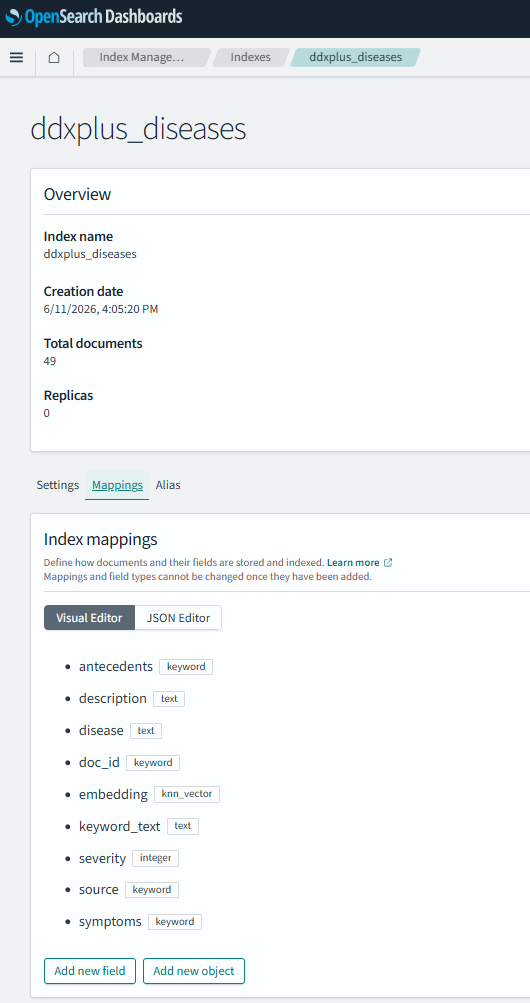
\includegraphics[width=0.42\textwidth]{Figures/ddxplus_mapping.png}
    \caption{Mapping chỉ mục \texttt{ddxplus\_diseases}: trường \texttt{keyword\_text} (\texttt{text}) phục vụ BM25, trường \texttt{embedding} (\texttt{knn\_vector}, 384 chiều, \texttt{cosinesimil}) phục vụ k-NN, đi kèm các metadata như \texttt{doc\_id}, \texttt{severity}, \texttt{description}\dots}
    \label{fig:os-mapping}
\end{figure}

\begin{figure}[H]
    \centering
    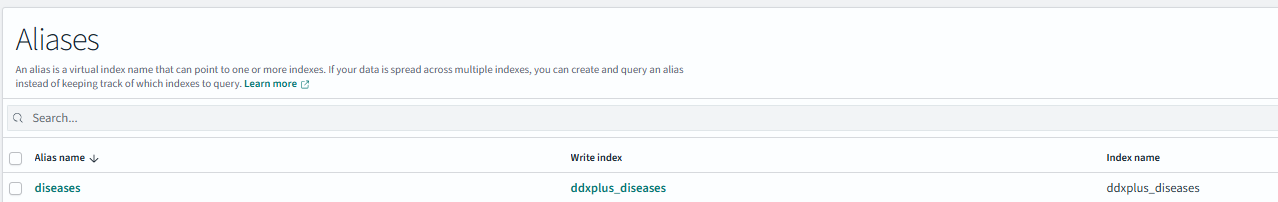
\includegraphics[width=0.95\textwidth]{Figures/alias.png}
    \caption{Bí danh (Alias) \texttt{diseases} trỏ tới chỉ mục vật lý hiện hành, cho phép \textit{swap} chỉ mục khi tiến hành tái lập (reindex) mà không làm rớt các yêu cầu truy vấn.}
    \label{fig:os-alias}
\end{figure}

\begin{figure}[H]
    \centering
    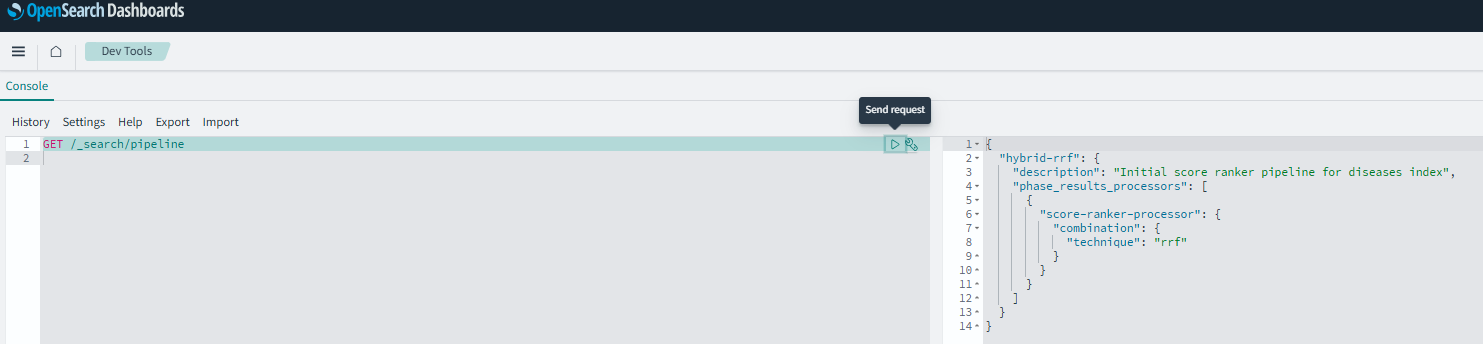
\includegraphics[width=0.95\textwidth]{Figures/phase_result_processor.png}
    \caption{Search pipeline \texttt{hybrid-rrf} tích hợp \texttt{score-ranker-processor} (sử dụng kỹ thuật \texttt{rrf}): hợp nhất thứ hạng của nhánh lexical (BM25) và nhánh semantic (k-NN) trực tiếp bên trong search engine.}
    \label{fig:os-pipeline}
\end{figure}

\subsection{Các chiến lược truy xuất: công thức và tham số}

\paragraph{BM25 (Okapi).}
BM25 được lựa chọn làm mô hình truy xuất từ vựng cốt lõi. Điểm số phù hợp giữa một truy vấn $Q$ và một tài liệu $D$ được định lượng theo công thức:
\begin{equation}
    \mathrm{BM25}(Q,D)=\sum_{t\in Q}\mathrm{IDF}(t)
    \cdot
    \frac{f(t,D)\,(k_1+1)}
    {f(t,D)+k_1\!\left(1-b+b\,\dfrac{|D|}{\mathrm{avgdl}}\right)},
\end{equation}
với thành phần tần số tài liệu nghịch đảo (IDF) được tính bằng:
\[
    \mathrm{IDF}(t)=
    \ln\!\left(
    1+\frac{N-n(t)+0.5}{n(t)+0.5}
    \right),
\]
trong đó $f(t,D)$ là tần suất xuất hiện của từ $t$ trong tài liệu, $|D|$ là độ dài tài liệu, $\mathrm{avgdl}$ là độ dài trung bình của toàn bộ tập tài liệu, $N$ đại diện cho tổng số tài liệu và $n(t)$ là số lượng tài liệu có chứa từ $t$.
Trong thiết lập thực nghiệm, hệ thống offline cấu hình BM25 với tham số $k_1=1.5$, $b=0.75$ kết hợp tokenizer \texttt{[a-z0-9]+}. Ngược lại, hệ thống production sử dụng cấu hình BM25 mặc định của OpenSearch ($k_1=1.2$, $b=0.75$) cùng với \textit{standard analyzer} trên trường \texttt{keyword\_text}. Truy vấn \texttt{match} được thực thi với toán tử \texttt{OR} (tài liệu được cộng điểm nếu chứa bất kỳ từ khoá nào có trong truy vấn). Hiệu năng của BM25 được đánh giá qua hai biến thể: truy vấn trên trường \texttt{keyword\_text} độc lập, và truy vấn trên trường \texttt{keyword\_text} kết hợp \texttt{description} (chi tiết xem tại mục Kết quả).

\paragraph{Dense Retrieval (k-NN).}
Dense Retrieval khai thác năng lực của mô hình \texttt{BAAI/bge-small-en-v1.5}~\cite{xiao2024cpack} để mã hoá cả truy vấn lẫn tài liệu thành không gian vector 384 chiều. Mức độ tương đồng về ngữ nghĩa được xác định qua hàm cosine:
\begin{equation}
    \mathrm{sim}(q,d)=\cos(\mathbf{v}_q,\mathbf{v}_d)
    =\frac{\mathbf{v}_q\cdot\mathbf{v}_d}
    {\lVert\mathbf{v}_q\rVert\,\lVert\mathbf{v}_d\rVert}.
\end{equation}
Vector của các tài liệu (đã được \textbf{chuẩn hoá L2}, do đó phép tính cosine tương đương với tích vô hướng dot-product) được sinh ra từ chuỗi ghép nối tên bệnh, triệu chứng và tiền sử trong khâu xây dựng KB. Hệ thống truy xuất production vận hành trên chỉ mục \texttt{knn\_vector} của OpenSearch (với cấu hình \texttt{space\_type=cosinesimil}, \texttt{index.knn=true}), sử dụng thuật toán tìm kiếm xấp xỉ HNSW~\cite{malkov2018hnsw} do engine Lucene cung cấp (tham số \texttt{ef\_construction}=100, \texttt{m}=16). Với quy mô Knowledge Base rất nhỏ chỉ gồm 49 tài liệu, kết quả tìm kiếm xấp xỉ gần như tiệm cận hoàn toàn với tìm kiếm vét cạn chính xác (exact k-NN); ưu thế về tốc độ của thuật toán HNSW chỉ thực sự phát huy khi quy mô tài liệu lớn hơn đáng kể. Số lượng lân cận truy xuất mặc định được thiết lập là $k=20$.

Điểm khác biệt trọng yếu giữa hai chế độ đánh giá (offline vs. production) nằm ở \textbf{cách biểu diễn chuỗi truy vấn} (tham khảo thêm về cách dùng tiền tố của họ mô hình BGE tại~\cite{xiao2024cpack}). Cụ thể: môi trường offline dựng chuỗi truy vấn dưới dạng câu tự nhiên \texttt{"Symptoms and antecedents: \dots"} và tiến hành mã hoá \textit{không} sử dụng tiền tố (prefix). Trong khi đó, môi trường production dùng hàm \texttt{embed\_query()} nối trực tiếp các token đã chuẩn hoá và gắn thêm tiền tố định hướng của BGE (\texttt{"Represent this sentence for searching relevant passages:"}). Sự bất đối xứng giữa truy vấn và tài liệu này được phân tích như nguyên nhân chính gây chênh lệch hiệu năng Dense Retrieval giữa hai chế độ ở mục Thảo luận.

\paragraph{Hybrid Retrieval (Reciprocal Rank Fusion).}
Hybrid Retrieval thực hiện việc phối hợp kết quả từ hai hướng truy xuất (BM25 và Dense Retrieval) dựa trên phương pháp \textit{Reciprocal Rank Fusion} (RRF):
\begin{equation}
    \mathrm{RRF}(d)=
    \sum_{r\in\{\mathrm{BM25},\,\mathrm{Dense}\}}
    \frac{1}{k+\mathrm{rank}_r(d)},
    \qquad
    k=60.
\end{equation}
Thay vì phải tìm cách chuẩn hoá và cộng gộp các thang điểm số (vốn rất khác biệt về mặt bản chất toán học giữa BM25 và Cosine), thuật toán RRF chỉ quan tâm đến \textit{vị trí thứ hạng} của tài liệu trong từng danh sách trả về, và \textbf{gán trọng số bằng nhau} cho cả nhánh BM25 lẫn Dense. Hằng số điều chuẩn $k=60$ là cấu hình mặc định của \texttt{score-ranker-processor}. Hệ thống offline tự thực hiện tính toán RRF trên hai mảng danh sách kết quả cục bộ, trong khi hệ thống production sử dụng truy vấn \texttt{hybrid} tích hợp \texttt{score-ranker-processor} gốc của OpenSearch. Cả hai hệ thống đều thiết lập trả về top-20 tài liệu.

\paragraph{Re-ranking và sinh câu trả lời.}
Bước sang Phase~2, 20 tài liệu được truy xuất sẽ trải qua khâu sắp xếp lại (re-ranking) bằng mô hình cross-encoder \texttt{bge-reranker-base}~\cite{xiao2024cpack}. Khác với kiến trúc bi-encoder (mã hoá truy vấn và tài liệu một cách \textit{độc lập} rồi mới tính toán khoảng cách cosine), kiến trúc cross-encoder sẽ \textbf{mã hoá đồng thời toàn bộ cặp (truy vấn, tài liệu)} xuyên qua một mạng Transformer. Quá trình này giúp mô hình nắm bắt tương tác chéo (cross-attention) mức từ vựng, mang lại điểm liên quan chính xác hơn, sau đó hệ thống giữ lại top-5 tài liệu cuối cùng (\texttt{RERANK\_TOP\_K}$=5$). Các tài liệu này được dùng làm ngữ cảnh truyền vào mô hình ngôn ngữ \texttt{Qwen3-8B}~\cite{qwen2025qwen3} để sinh ra câu trả lời tự nhiên. Tại thời điểm báo cáo, mã nguồn cho phần re-ranking đã hoàn tất, nhưng việc phân tích và đánh giá các chỉ số định lượng liên quan được lên kế hoạch cho Phase~2.

\subsection{Hai chế độ đánh giá: in-memory offline và OpenSearch production}

Với mục tiêu đánh giá khách quan chất lượng của các chiến lược truy xuất, đồng thời tách biệt ảnh hưởng của hạ tầng triển khai, nhóm nghiên cứu đã thiết lập hai bộ khai thác (harness) chạy song song trên cùng một Knowledge Base, dùng chung một pipeline tiền xử lý và đo lường trên cùng một bộ dữ liệu gán nhãn. Hai chế độ này chỉ khác biệt về lõi thực thi (execution engine), được tóm tắt chi tiết trong Bảng~\ref{tab:harness}.

\begin{enumerate}[leftmargin=1.4em,itemsep=2pt]
    \item \textbf{Offline (in-memory).} Toàn bộ logic truy xuất được lập trình và chạy hoàn toàn bằng Python, độc lập hoàn toàn với OpenSearch. BM25 được cài đặt bám sát công thức lý thuyết Okapi ($k_1=1.5$, $b=0.75$), Dense Retrieval sử dụng thư viện \texttt{sentence-transformers} nạp mô hình \texttt{BAAI/bge-small-en-v1.5}~\cite{xiao2024cpack}, và Hybrid Retrieval tính toán RRF ($k=60$) thủ công. Do Knowledge Base có quy mô nhỏ (49 tài liệu), việc tính toán brute-force trên toàn bộ tập dữ liệu có chi phí tính toán thấp, đủ để làm mốc tham chiếu cho chất lượng của các thuật toán truy xuất.
    \item \textbf{Production (OpenSearch).} Knowledge Base được nạp (ingest) thực tế vào OpenSearch thông qua API, trải qua quy trình chuẩn hoá, sinh vector và bulk indexing thực thụ. Các tác vụ tìm kiếm được gọi qua giao thức RESTful sử dụng \texttt{match} (BM25), \texttt{knn} (Dense) và \texttt{hybrid} (RRF pipeline). Đây chính là mô hình phản ánh đúng cấu hình của hệ thống production đang chạy phục vụ người dùng cuối.
\end{enumerate}

\paragraph{Xây dựng truy vấn và nhãn đánh giá.}
Chuỗi truy vấn của mỗi bệnh nhân được xây dựng từ trường \texttt{EVIDENCES} thông qua các bước làm sạch nghiêm ngặt: cắt bỏ các hậu tố giá trị cụ thể (\texttt{\_@\_<value>}), ánh xạ từng mã hệ thống thành cụm từ y khoa thông qua hàm \texttt{normalize\_symptom\_phrase}, khử trùng lặp và cuối cùng là nối thành câu truy vấn. Tên của bệnh (chẩn đoán cuối cùng) bị loại bỏ hoàn toàn khỏi truy vấn để ngăn chặn triệt để hiện tượng rò rỉ dữ liệu nhãn (data leakage). Nhãn đúng được lấy từ trường \texttt{PATHOLOGY} của bộ dữ liệu gốc DDXPlus.

\paragraph{Chỉ số đánh giá.}
Hệ thống sử dụng một bộ các chỉ số đo lường học thuật tiêu chuẩn trong Information Retrieval, bao gồm Hit@1, Hit@3, Hit@5 và Mean Reciprocal Rank (MRR), trong đó Hit@1 được định vị là chỉ số tối quan trọng (primary metric). Bản chất toán học của chúng như sau:
\begin{itemize}[leftmargin=1.4em,itemsep=2pt]
    \item \textbf{Hit@$k$} (Tỉ lệ trúng đích trong top-$k$): Trả về giá trị nhị phân $1$ nếu tài liệu chứa bệnh lý kỳ vọng nằm gọn trong top $k$ tài liệu trả về đầu tiên, ngược lại nhận giá trị $0$. Giá trị tổng quát được tính bằng giá trị trung bình trên toàn bộ tập truy vấn. \textbf{Hit@1} đánh giá năng lực dự đoán trúng đích ở ngay vị trí số 1 (mô phỏng tình huống hệ thống tự động đưa ra một chẩn đoán duy nhất). \textbf{Hit@3} và \textbf{Hit@5} thể hiện khả năng hệ thống cung cấp một danh sách ngắn gọn nhưng chứa đựng chẩn đoán đúng để bác sĩ chuyên môn tiến hành loại trừ (differential diagnosis).
    \item \textbf{MRR} (Mean Reciprocal Rank): Là trung bình cộng của nghịch đảo thứ hạng ($1/\mathrm{rank}$) của tài liệu chứa bệnh đúng đối với mọi truy vấn. (Trường hợp tài liệu đúng hoàn toàn không xuất hiện, giá trị nghịch đảo bằng $0$). Không giống Hit@$k$ chỉ mang tính nhị phân "có/không", MRR là một chỉ số liên tục, thưởng điểm cao hơn khi tài liệu đúng đứng ở \textit{những vị trí càng cao}, do đó nó nhạy hơn trong việc phản ánh chất lượng xếp hạng tinh hơn. Trong nghiên cứu này, MRR được tính trượt trên toàn vẹn 49 tài liệu (không bị áp dụng cắt tỉa ngưỡng top-$k$).
\end{itemize}
Mặt khác, do không gian đáp án chỉ gói gọn trong 49 tài liệu, đường cơ sở xác suất nếu chọn ngẫu nhiên (random guess baseline) của các chỉ số này (với Hit@1 $\approx 2\%$) sẽ được làm rõ hơn trong phần Dữ liệu và thiết lập thí nghiệm.
\section{Dữ liệu và thiết lập thí nghiệm (Experiments)}
% [NHÁP -- Dataset: Hoàng Phước Nguyên & Thương (KB); Thiết lập đánh giá: Thương.]

\subsection{Dataset}
\begin{itemize}
\item \textbf{Tên dataset:} DDXPlus~\cite{ddxplus2022} (English), \textbf{phiên bản 2 -- đăng ngày 10/03/2026} trên Figshare; giấy phép CC-BY.
\item \textbf{Quy mô tri thức:} \textbf{49 bệnh} (\texttt{release\_conditions.json}) và \textbf{223 bằng chứng triệu chứng} (\texttt{release\_evidences.json}); kèm mã ICD-10 và mức độ nặng (severity, thang 1--5, 1 là nặng nhất).
\item \textbf{Quy mô bệnh nhân:} khoảng 1,3 triệu hồ sơ bệnh nhân tổng hợp (synthetic), chia train/validate/test.
\item \textbf{KB:} mỗi bệnh là một tài liệu mô tả bằng tập evidence (trường \texttt{keyword\_text}, \texttt{embedding} 384 chiều, \texttt{symptoms}, \texttt{disease}, \texttt{icd10\_codes}, \texttt{severity}).
\item \textbf{Xử lý dữ liệu (rà soát KB -- PR \#6):} chuẩn hoá token evidence dùng chung normalizer build/query; bổ sung \texttt{icd10\_codes}; sửa Pneumonia J17 $\rightarrow$ J18; tái sinh KB (49 tài liệu, 0 token lệch).
\item \textbf{Trường \texttt{description}:} mô tả do nhóm tự tổng hợp (ghép chuỗi từ triệu chứng); nhóm thống nhất index đầy đủ các trường trong mapping để Phase 2 (inject ngữ cảnh cho LLM) tái sử dụng được, không phải dựng lại.
\end{itemize}

\subsection{Chia dữ liệu}
Sử dụng phân chia gốc train/validate/test của DDXPlus (stratified). KB được xây từ \textit{định nghĩa bệnh}; truy vấn lấy từ \textit{evidences của bệnh nhân}; tên bệnh (nhãn gold) bị loại khỏi truy vấn để tránh rò rỉ thông tin (data leakage). Đánh giá truy xuất offline được thực hiện trên \textbf{toàn bộ tập validate ($n=132{,}448$)}. Nhóm cũng khử trùng dòng trong bộ eval (nhật ký: test 101, validate 75; \texttt{scripts/dedup\_eval.py}, \texttt{data/kb/dedup\_eval\_log.md}).

\subsection{Thiết lập huấn luyện}
Nghiên cứu \textbf{không fine-tune}; dùng embedding pretrained \texttt{BAAI/bge-small-en-v1.5} (384 chiều, cosine) theo dạng zero-shot.

\subsection{Thiết lập đánh giá và quy ước đối chiếu}
\begin{itemize}
\item \textbf{Metric chính:} Hit@1. \textbf{Metric phụ:} Hit@3, Hit@5, MRR@5; Tier-1 còn bổ sung NDCG@5.
\item \textbf{Chế độ offline (Python thuần):} EXP-01 (BM25 tham chiếu) và EXP-02 (Dense, Hybrid-RRF) chạy trên toàn bộ $n=132{,}448$; Okapi BM25 ($k_1=1.5$, $b=0.75$, tokenizer \texttt{[a-z0-9]+}), tie-break tất định.
\item \textbf{Chế độ live (OpenSearch):} ingest KB rồi truy xuất qua BM25 + k-NN + search pipeline \texttt{hybrid-rrf}. Lần chạy thử ngày \textbf{25/06/2026} dùng \textbf{mẫu 5.000 bệnh nhân, seed 13} (đồng bộ cách lấy mẫu với EXP-02); lần chạy đầy đủ ($n=132{,}448$, ước tính 30--60 phút) \textbf{đang được Tú thực hiện để hoàn tất đánh giá Phase 1}.
\item \textbf{Nguyên tắc so sánh:} cùng KB, cùng normalizer, cùng ground truth; chỉ khác hạ tầng. Bảng đối chiếu (mục Kết quả) trình bày song song để đo độ sai khác giữa hai chế độ.
\end{itemize}

\begin{figure}[H]
\centering
\fbox{\begin{minipage}{0.92\textwidth}\centering\vspace{1.0cm}\textit{[Chỗ dành cho hình -- cần \textbf{Tú} (hoặc \textbf{Trí}) bổ sung: ảnh chụp OpenSearch Dashboards minh hoạ chỉ mục KB, alias \texttt{diseases} và search pipeline \texttt{hybrid-rrf}.]}\vspace{1.0cm}\end{minipage}}
\caption{Minh hoạ hạ tầng OpenSearch (do thành viên bổ sung để hoàn tất Phase 1).}
\end{figure}
\section{Kết quả thí nghiệm (Results)}
% [SỐ LIỆU THỰC -- EXP-02 offline (19/06, n=132,448) + OpenSearch live (25/06, mẫu 5.000, seed 13). Trình bày: Hương; số liệu: Thương/Tú.]

\subsection{Kết quả tham chiếu offline (Python thuần, n=132,448)}
Bảng \ref{tab:offline} tổng hợp kết quả EXP-01/EXP-02 chạy bằng Python thuần trên toàn bộ tập validate. Các dòng BM25 là tham chiếu từ EXP-01; đóng góp của EXP-02 là Dense và Hybrid-RRF.

\begin{table}[H]
\centering
\small
\caption{Kết quả truy xuất offline (Python thuần) trên tập validate DDXPlus đầy đủ ($n=132{,}448$). Dense: \texttt{bge-small-en-v1.5}; Hybrid: RRF($k=60$).}
\label{tab:offline}
\begin{tabular}{lcccc}
\hline
\textbf{Phương pháp} & \textbf{Hit@1} & \textbf{Hit@3} & \textbf{Hit@5} & \textbf{MRR}\\
\hline
BM25 + description \textit{(EXP-01)} & \textbf{98.78\%} & 99.96\% & 100.00\% & \textbf{0.9937}\\
BM25 keyword\_text \textit{(EXP-01)} & 98.47\% & 99.95\% & 99.99\% & 0.9921\\
Hybrid-RRF + description & 91.95\% & 99.52\% & 99.77\% & 0.9570\\
Hybrid-RRF (no-desc) & 91.17\% & 98.89\% & 99.61\% & 0.9511\\
Dense + description & 84.28\% & 95.48\% & 98.46\% & 0.9027\\
Dense (no-desc) & 83.11\% & 94.41\% & 96.82\% & 0.8911\\
\hline
\end{tabular}
\end{table}

\begin{figure}[H]
\centering
\begin{tikzpicture}
\begin{axis}[
  ybar, bar width=9pt,
  width=0.92\textwidth, height=6.2cm,
  enlarge x limits=0.28,
  ymin=80, ymax=103,
  ylabel={Tỉ lệ (\%)},
  symbolic x coords={BM25, Hybrid-RRF, Dense},
  xtick=data,
  legend style={at={(0.5,-0.18)}, anchor=north, legend columns=3, font=\footnotesize},
]
\addplot coordinates {(BM25,98.78) (Hybrid-RRF,91.95) (Dense,84.28)};
\addplot coordinates {(BM25,99.96) (Hybrid-RRF,99.52) (Dense,95.48)};
\addplot coordinates {(BM25,100.00) (Hybrid-RRF,99.77) (Dense,98.46)};
\legend{Hit@1, Hit@3, Hit@5}
\end{axis}
\end{tikzpicture}
\caption{So sánh Hit@1/Hit@3/Hit@5 của ba chiến lược (cấu hình + description, offline Python thuần, $n=132{,}448$).}
\label{fig:bar}
\end{figure}

\textbf{Nhận xét (offline):} thứ tự Hit@1 là \textbf{BM25 (98.78\%) $>$ Hybrid (91.95\%) $>$ Dense (84.28\%)} -- BM25 hơn Hybrid 6.83 điểm \%, hơn Dense 14.50 điểm \%. Trường \textit{description} cải thiện đều cả ba (Dense +1.17, Hybrid +0.78, BM25 +0.31 điểm \% Hit@1); trong RRF, thành phần BM25 đang đóng góp chính.

\subsection{Đối chiếu Python thuần với OpenSearch (mẫu 5.000, seed 13)}
Ngày 25/06/2026, nhóm chạy thử pipeline OpenSearch live trên \textbf{mẫu 5.000 bệnh nhân (seed 13)} -- cùng cách lấy mẫu với EXP-02 -- để kiểm chứng tính nhất quán giữa hai hạ tầng (Bảng \ref{tab:livevsoffline}). So sánh dùng biến thể \texttt{keyword\_text} ở cả hai chế độ.

\begin{table}[H]
\centering
\small
\caption{Đối chiếu OpenSearch live (mẫu 5.000, seed 13) với Python thuần (offline, đầy đủ), biến thể \texttt{keyword\_text}.}
\label{tab:livevsoffline}
\begin{tabular}{llccccr}
\hline
\textbf{Phương pháp} & \textbf{Hạ tầng} & \textbf{Hit@1} & \textbf{Hit@3} & \textbf{Hit@5} & \textbf{MRR} & \textbf{$n$}\\
\hline
BM25 & OpenSearch live & 98.88\% & 99.96\% & 99.98\% & 0.9942 & 5.000\\
BM25 & Python thuần & 98.47\% & 99.95\% & 99.99\% & 0.9921 & 132.448\\
Hybrid-RRF & OpenSearch live & 92.50\% & 98.86\% & 99.52\% & 0.9575 & 5.000\\
Hybrid-RRF & Python thuần & 91.17\% & 98.89\% & 99.61\% & 0.9511 & 132.448\\
\hline
\end{tabular}
\end{table}

\textbf{Nhận xét (đối chiếu):} hai hạ tầng cho kết quả \textbf{rất nhất quán}: chênh lệch Hit@1 chỉ +0.41 điểm \% (BM25) và +1.33 điểm \% (Hybrid) theo hướng live cao hơn, nằm trong dao động do cỡ mẫu 5.000 và khác biệt cài đặt engine (analyzer, tie-break, k-NN xấp xỉ HNSW). Quan trọng hơn, \textbf{thứ tự BM25 $>$ Hybrid được bảo toàn}, khẳng định bộ số offline là mốc tham chiếu/trần trên hợp lệ cho logic truy xuất. Con số chốt cuối vẫn lấy từ lần chạy OpenSearch đầy đủ (Bảng \ref{tab:livefull}).

\subsection{Kết quả OpenSearch chạy đầy đủ (Tú cập nhật sau khi chạy full)}
Bảng \ref{tab:livefull} là khung số liệu \textit{production} trên toàn tập validate -- \textbf{con số chốt của Phase 1} -- do \textbf{Nguyễn Minh Tú} điền sau khi chạy pipeline OpenSearch đầy đủ ($n=132{,}448$, ước tính 30--60 phút). Khi điền, ghi kèm cột $\Delta$ so với offline tương ứng để soi độ sai khác hạ tầng.

\begin{table}[H]
\centering
\small
\caption{Kết quả OpenSearch đầy đủ -- \textit{khung chờ điền (Người điền: Nguyễn Minh Tú)}.}
\label{tab:livefull}
\begin{tabular}{lcccccr}
\hline
\textbf{Phương pháp} & \textbf{Hit@1} & \textbf{Hit@3} & \textbf{Hit@5} & \textbf{MRR} & \textbf{NDCG@5} & \textbf{$n$}\\
\hline
BM25 (keyword\_text) & \textit{[Tú điền]} & \textit{[..]} & \textit{[..]} & \textit{[..]} & \textit{[..]} & 132.448\\
BM25 + description & \textit{[Tú điền]} & \textit{[..]} & \textit{[..]} & \textit{[..]} & \textit{[..]} & 132.448\\
Hybrid-RRF & \textit{[Tú điền]} & \textit{[..]} & \textit{[..]} & \textit{[..]} & \textit{[..]} & 132.448\\
Dense & \textit{[Tú điền]} & \textit{[..]} & \textit{[..]} & \textit{[..]} & \textit{[..]} & 132.448\\
+ Reranker (A4, Phase 2) & \textit{[Tú điền]} & \textit{[..]} & \textit{[..]} & \textit{[..]} & \textit{[..]} & 132.448\\
\hline
\end{tabular}
\end{table}

\subsection{Chỉ số QA bổ sung (tùy chọn)}
Bảng \ref{tab:qa} dành cho \textbf{Nguyễn Thị Diễm Hương} bổ sung các chỉ số QA theo phần research (nếu muốn), giúp đánh giá toàn diện hơn ngoài Hit@k/MRR.

\begin{table}[H]
\centering
\small
\caption{Chỉ số QA bổ sung -- \textit{khung chờ điền (Người điền: Nguyễn Thị Diễm Hương)}.}
\label{tab:qa}
\begin{tabular}{p{6.2cm}p{3.2cm}p{2.4cm}}
\hline
\textbf{Chỉ số QA} & \textbf{Ý nghĩa} & \textbf{Giá trị}\\
\hline
NDCG@5 (graded relevance) & Chất lượng xếp hạng có trọng số & \textit{[Hương điền]}\\
Tier-1.5: ICD-10 chapter Hit@1 & Đúng chương ICD-10 & \textit{[Hương điền]}\\
Tier-1.5: ICD-10 block Hit@1 & Đúng block ICD-10 & \textit{[Hương điền]}\\
MSR (Missed-Severe Ratio, severity $\le 2$) & Tỉ lệ bỏ sót bệnh nặng & \textit{[Hương điền]}\\
Bootstrap 95\% CI (B=1000, seed 42) & Khoảng tin cậy của Hit@1 & \textit{[Hương điền]}\\
\hline
\end{tabular}
\end{table}

\begin{notebox}{Quy ước điền số liệu}
\begin{itemize}
\item Bảng 1--2: số liệu đã chốt (offline + đối chiếu mẫu 5k) -- KHÔNG sửa.
\item Bảng 3: Nguyễn Minh Tú điền sau khi chạy OpenSearch đầy đủ; ghi rõ ngày chạy, seed, và $\Delta$ so với offline.
\item Bảng 4: Nguyễn Thị Diễm Hương điền các chỉ số QA tùy chọn; nêu rõ công thức nếu khác chuẩn.
\item Mọi con số phải kèm $n$ (cỡ mẫu) và làm tròn 2 chữ số thập phân để so sánh được.
\end{itemize}
\end{notebox}
\section{Ablation Study và phân tích bổ sung}
% [NHÁP -- Phụ trách: Nguyễn Thị Diễm Hương & Nguyễn Minh Tú.]

\textbf{(A) Ảnh hưởng của trường \textit{description} (A/B):} bật \textit{description} cải thiện Hit@1 ở cả ba phương pháp -- Dense +1.17, Hybrid +0.78, BM25 +0.31 điểm \% -- cho thấy \textit{description} cung cấp tín hiệu hữu ích và nhất quán; nên giữ ở cả keyword text lẫn embedding.

\textbf{(B) Ảnh hưởng của chiến lược truy xuất:} trên bộ đánh giá hiện tại, lexical (BM25) chiếm ưu thế; hybrid kéo theo thành phần BM25 nên cao hơn dense thuần (Bảng \ref{tab:offline}).

\textbf{(C) Tính nhất quán hạ tầng (offline vs OpenSearch):} trên toàn tập ($n=132{,}448$), chênh lệch Hit@1 giữa Python thuần và OpenSearch live nhỏ ở BM25/Hybrid ($+0.18$/$+1.13$ điểm \%) và giữ nguyên thứ hạng phương pháp (Bảng \ref{tab:livevsoffline}), củng cố độ tin cậy của logic truy xuất.

\textbf{(D) Phân tích dự kiến (Phase 2):} (i) tinh chỉnh trọng số RRF (tăng tỉ trọng BM25 hoặc cascade BM25 $\rightarrow$ dense khi top-1 thiếu tự tin); (ii) thay embedding y khoa chuyên biệt; (iii) thêm re-ranking. Mục tiêu là kiểm chứng giá trị của kiến trúc hai tầng trên truy vấn ngôn ngữ tự nhiên.
\section{Thảo luận (Discussion)}
% [NHÁP -- Phụ trách: cả nhóm; chủ trì: Nguyễn Văn Thương.]

\textbf{Vì sao BM25 dẫn đầu trên bộ đánh giá này?} Truy vấn được tạo từ các token evidence \textit{đã chuẩn hoá}, trùng khớp từ vựng cao với KB -- điều kiện thuận lợi cho khớp từ chính xác của BM25. Do đó kết quả \textbf{không} đồng nghĩa với việc kiến trúc dense/hybrid kém hơn về bản chất.

\textbf{Vai trò của description:} cải thiện đều cả ba phương pháp, củng cố quyết định giữ trường này.

\textbf{Python thuần so với OpenSearch:} bộ số offline được thiết kế như một mốc tham chiếu/trần trên cho logic truy xuất; lần chạy OpenSearch live (mẫu 5k) cho kết quả nhất quán cả về giá trị lẫn thứ hạng, nên có thể tin cậy chuyển sang đo production đầy đủ. Khác biệt nhỏ giữa hai hạ tầng đến từ analyzer của OpenSearch, cơ chế tie-break và k-NN xấp xỉ (HNSW) so với cosine brute-force.

\textbf{Hệ quả thiết kế:} (i) embedding phổ thông (không chuyên y khoa) chưa được kiểm tra đúng thế mạnh ngữ nghĩa; (ii) RRF cào bằng trọng số kéo lùi BM25 gần hoàn hảo; (iii) cần bộ truy vấn ngôn ngữ tự nhiên để đo đúng giá trị dense/hybrid. Các điểm này định hướng cho Phase 2.
\section{Phân tích lỗi và hạn chế}
% [NHÁP -- Phụ trách: Nguyễn Thị Diễm Hương (phân tích lỗi) & Nguyễn Văn Thương (hạn chế).]

\textbf{Các bệnh khó nhất (offline, biến thể keyword\_text):} một số bệnh có Hit@1 thấp rõ rệt do chồng lấp triệu chứng và mô tả ngắn (Bảng \ref{tab:hard}). Lần chạy OpenSearch live (mẫu 5k) cho cùng xu hướng: Acute rhinosinusitis và Unstable angina vẫn là hai bệnh khó nhất.

\begin{table}[H]
\centering
\small
\caption{Các bệnh có Hit@1 thấp nhất (offline, keyword\_text, $n$ theo từng bệnh).}
\label{tab:hard}
\begin{tabular}{lcc}
\hline
\textbf{Bệnh} & \textbf{Hit@1} & \textbf{$n$}\\
\hline
Acute rhinosinusitis & 49.62\% & 1.866\\
Unstable angina & 84.32\% & 2.748\\
Myocarditis & 93.54\% & 1.547\\
Bronchitis & 96.87\% & 3.543\\
URTI & 97.78\% & 8.656\\
SLE & 97.97\% & 1.579\\
Stable angina & 98.25\% & 2.340\\
\hline
\end{tabular}
\end{table}

\textbf{Kiểm chứng hồi quy KB (PR \#6):} 9/49 bệnh từng bị ảnh hưởng bởi lệch normalizer (Anemia, Bronchiectasis, Cluster headache, GERD, Guillain-Barré syndrome, Localized edema, Panic attack, Pulmonary embolism, Tuberculosis) sau khi sửa đều đạt 99--100\% Hit@1 -- không gây hồi quy.

\begin{figure}[H]
\centering
\fbox{\begin{minipage}{0.92\textwidth}\centering\vspace{1.0cm}\textit{[Chỗ dành cho hình -- cần \textbf{Hương} bổ sung: biểu đồ phân tích lỗi / ma trận nhầm lẫn cho các bệnh chồng lấp triệu chứng (vd Acute rhinosinusitis, Unstable angina).]}\vspace{1.0cm}\end{minipage}}
\caption{Phân tích lỗi định tính (do QA bổ sung).}
\end{figure}

\textbf{Hạn chế của nghiên cứu:}
\begin{itemize}
\item \textbf{Thiết kế đánh giá thiên lexical:} truy vấn chuẩn hoá trùng KB, có lợi cho BM25; chưa đánh giá trên truy vấn ngôn ngữ tự nhiên/nhiễu.
\item \textbf{Embedding phổ thông:} \texttt{bge-small-en-v1.5} chưa chuyên biệt cho y khoa.
\item \textbf{RRF chưa tinh chỉnh trọng số.}
\item \textbf{Phạm vi OpenSearch:} mới chạy live trên \textbf{mẫu 5.000} (seed 13); lần chạy đầy đủ ($n=132{,}448$, 30--60 phút) còn lại cho Phase 2.
\item \textbf{Cấu phần chưa triển khai:} re-ranking (A4) và sinh câu trả lời bằng LLM (A5) thuộc Phase 2.
\item \textbf{Số lần chạy:} báo cáo một lần chạy trên toàn tập do hạn chế tài nguyên; cần bootstrap CI để khẳng định ý nghĩa thống kê.
\end{itemize}
\section{Kế hoạch Phase 2 (Module 2)}
% [NHÁP -- Chủ trì: Nguyễn Văn Thương; pipeline: Tú/Trí; QA: Hương.]

Phase 1 đã chốt Thiết kế A (DDXPlus-only, retrieval-first) với không gian nhãn duy nhất gồm 49 bệnh, KB đã chuẩn hoá và kiểm định, bộ số offline (Python thuần) làm trần trên, và lần chạy OpenSearch đầy đủ ($n=132{,}448$, 26/06/2026) xác nhận tính nhất quán và chốt số production cho Phase 1 (BM25 và Hybrid bám sát offline; Dense lệch do khác biệt prefix khi embed truy vấn). Phase 2 hoàn thiện hệ thống end-to-end trên hạ tầng thật và bổ sung sinh câu trả lời.

\textbf{Chiến lược trên DDXPlus:} giữ truy xuất làm lõi (retrieval-first), nâng dần theo bậc A1 BM25 $\rightarrow$ A2 k-NN $\rightarrow$ A3 Hybrid-RRF (đã chốt ở Phase 1) $\rightarrow$ A4 + reranker (\textit{mã nguồn cuối Phase 1, đánh giá Phase 2}) $\rightarrow$ A5 sinh câu trả lời (Module 2, Phase 2). Mọi bước được đo trên cùng KB + normalizer để so sánh công bằng với bộ offline.

\begin{figure}[H]
    \centering
    \resizebox{\textwidth}{!}{%
        \begin{tikzpicture}[node distance=1.0cm]
            \node[stage, text width=3.0cm] (p1) {\textbf{Phase 1 (MVP)}\\KB chuẩn hoá + offline (Python) + production full 132k + reranker (mã nguồn)};
            \node[future, text width=3.0cm, right=of p1] (f1) {\textbf{Phase 2 -- Đánh giá nâng cao}\\đánh giá A4 reranker + Tier-1.5 + truy vấn NL + đồng bộ prefix + bootstrap CI};
            \node[future, text width=3.0cm, right=of f1] (g1) {\textbf{Phase 2 -- Module 2}\\A5 Qwen3-8B + FastAPI};
            \draw[flow] (p1) -- (f1);
            \draw[flow] (f1) -- (g1);
        \end{tikzpicture}}
    \caption{Lộ trình Phase 1 $\rightarrow$ Phase 2 trên DDXPlus (retrieval-first).}
    \label{fig:roadmap}
\end{figure}

\begin{table}[H]
    \centering
    \small
    \caption{Hạng mục Phase 2, người phụ trách và metric chốt.}
    \label{tab:phase2}
    \begin{tabular}{p{4.3cm}p{4.0cm}p{3.4cm}}
        \hline
        \textbf{Hạng mục}                                                                                                  & \textbf{Phụ trách}                         & \textbf{Metric / đầu ra}          \\
        \hline
        Hoàn thiện \texttt{ingest.py} + index (alias \texttt{diseases}); khớp KB (antecedents, icd10\_codes)               & Vương Đình Minh Trí (critical path)        & 49 docs trên engine, 0 token lệch \\
        \textbf{Đồng bộ prefix BGE} offline $\leftrightarrow$ production khi embed truy vấn; tái đo Dense/Hybrid           & Nguyễn Minh Tú + Nguyễn Văn Thương         & đối chiếu Dense công bằng         \\
        Đánh giá A4 re-ranking \textit{(mã nguồn đã merge ở Phase 1)} (\texttt{bge-reranker-base}, top20$\rightarrow$top5) & Nguyễn Minh Tú                             & $\Delta$ so với A3                \\
        Sinh câu trả lời A5 (\texttt{Qwen3-8B}) + FastAPI                                                                  & Nguyễn Minh Tú                             & chất lượng câu trả lời            \\
        Bộ truy vấn ngôn ngữ tự nhiên (thiếu/nhiễu triệu chứng)                                                            & Nguyễn Thị Diễm Hương + Hoàng Phước Nguyên & đo đúng dense/hybrid              \\
        Tier-1.5: NDCG@5 + Hit@1 theo chương/block ICD-10 \textit{(cần dự đoán per-case)}                                                      & Nguyên + Hương + Thương                    & an toàn lâm sàng                  \\
        Bootstrap CI 95\% (B=1000, seed 42) trên số production                                                             & Nguyễn Văn Thương + Tú                     & CI 95\% cho Hit@1                 \\
        \hline
    \end{tabular}
\end{table}

\textbf{Tiêu chí hoàn thành Phase 2:} (i) Dense/Hybrid được đo lại sau khi đồng bộ quy ước prefix; (ii) A4 cho cải thiện đo được so với A3; (iii) A5 sinh câu trả lời có trích dẫn nguồn; (iv) chạy TEST 1 lần duy nhất để báo cáo cuối.

\section{Thiết lập và vận hành nhóm}
% [NHÁP -- Chủ trì: Nguyễn Văn Thương (quản lý) & Vương Đình Minh Trí (DevOps).]

Nhóm vận hành trên bốn công cụ, mỗi công cụ một vai trò rõ ràng, kết nối bằng đồng bộ tự động để tránh nhập tay trùng lặp:
\begin{itemize}
    \item \textbf{JIRA} (key SCRUM) -- điểm tạo và quản lý công việc (Scrum board, sprint): \url{https://thng.atlassian.net/jira/software/projects/SCRUM/boards/1}.
    \item \textbf{Notion} -- Single Source of Truth: tài liệu, kế hoạch, ADR, log thí nghiệm, knowledge hub (không gian làm việc nội bộ của nhóm).
    \item \textbf{Discord} (server ID \texttt{1511918814995157074}) -- kênh trao đổi và nhận thông báo tự động.
    \item \textbf{GitHub} -- mã nguồn, Pull Request, review (\texttt{Disease-Diagnosis-RAG-System}).
\end{itemize}

\begin{figure}[H]
    \centering
    \resizebox{0.95\textwidth}{!}{%
        \begin{tikzpicture}
            % --- Nút đặt bằng toạ độ tuyệt đối để tránh chồng lấp ---
            \node[stage, text width=2.6cm] (notion)  at (0,1.5)   {\textbf{Notion}\\Source of Truth};
            \node[stage, text width=2.6cm] (jira)    at (-5.2,1.5) {\textbf{JIRA}\\Scrum board};
            \node[stage, text width=2.6cm] (discord) at (5.2,1.5)  {\textbf{Discord}\\Thông báo nhóm};
            \node[stage, text width=2.6cm] (github)  at (0,3.7)   {\textbf{GitHub}\\Code + PR};
            \node[future, text width=2.6cm] (prism)   at (0,-0.5)  {\textbf{Prism/Overleaf}\\Báo cáo};
            % --- Mũi tên ---
            \draw[twoway] (jira) -- node[above, font=\footnotesize, align=center]{Unito\\2 chiều} (notion);
            \draw[flow] (github) -- node[right, font=\footnotesize]{evidence/PR} (notion);
            \draw[flow] (notion) -- node[right, font=\footnotesize]{nội dung} (prism);
            % Kênh thông báo JIRA -> Discord đi vòng dưới (Manhattan), nằm hẳn dưới Prism
            \draw[flow] (jira.south) |- (0,-2.6) -| (discord.south);
            \node[font=\footnotesize, align=center] at (0,-2.95) {Jira Automation, 1 chiều};
        \end{tikzpicture}}
    \caption{Sơ đồ đồng bộ công cụ: JIRA $\leftrightarrow$ Notion (2 chiều, Unito), JIRA $\rightarrow$ Discord (1 chiều, Jira Automation). Notion và Discord không đồng bộ trực tiếp.}
    \label{fig:toolchain}
\end{figure}

\subsection{Đồng bộ JIRA $\leftrightarrow$ Notion (Unito, 2 chiều)}
\begin{table}[H]
    \centering
    \small
    \caption{Sáu trường đồng bộ hai chiều giữa JIRA và Notion (Unito).}
    \label{tab:unito}
    \begin{tabular}{lll}
        \hline
        \textbf{JIRA}        & \textbf{Notion} & \textbf{Chiều}     \\
        \hline
        Summary              & Task Name       & 2 chiều            \\
        Status               & Status          & 2 chiều            \\
        Priority             & Priority        & 2 chiều            \\
        Sprint               & Sprint          & 2 chiều            \\
        Due date             & Deadline        & 2 chiều            \\
        Description (footer) & Link            & 1 chiều (gắn link) \\
        \hline
    \end{tabular}
\end{table}

\subsection{Thông báo JIRA $\rightarrow$ Discord (Jira Automation, 1 chiều)}
Sáu luồng thông báo tự động gửi qua webhook vào kênh Discord (Webhook \#1 và \#2 theo loại sự kiện):
\begin{enumerate}
    \item Tạo issue mới (issue created).
    \item Đổi trạng thái (status changed).
    \item Đổi người phụ trách (assignee changed).
    \item Thêm bình luận (comment added).
    \item Bắt đầu / kết thúc sprint.
    \item Hoàn thành issue (done).
\end{enumerate}
\textit{Lưu ý bảo mật:} không in URL webhook đầy đủ trong tài liệu; chỉ cấu hình trong JIRA Automation.

\textbf{Nguyên tắc:} Notion là nguồn sự thật cho tài liệu; JIRA là nguồn sự thật cho công việc; mọi task chỉ tạo ở một nơi (JIRA) rồi đồng bộ sang Notion; Discord chỉ nhận thông báo một chiều. Phiên bản JIRA miễn phí giới hạn 10 người dùng; quản trị: Nguyễn Văn Thương.

\section{Tái lập kết quả và mã nguồn (Replicate the results)}

Để đảm bảo khả năng tái lập kết quả, toàn bộ mã nguồn, tài liệu hướng dẫn và các thành phần triển khai của hệ thống được quản lý tập trung trên GitHub. Dự án sử dụng môi trường Python cùng OpenSearch làm cơ sở dữ liệu vector và BM25, đồng thời áp dụng quy trình kiểm thử tự động nhằm đảm bảo tính ổn định của hệ thống trước khi thực hiện các thí nghiệm.

\subsection{Mã nguồn và cấu trúc dự án}

Mã nguồn của dự án được công khai tại:

\begin{center}
\url{https://github.com/AIVIETNAM-AIO-Lucyna/Disease-Diagnosis-RAG-System}
\end{center}

Nhánh phát triển chính của dự án là \texttt{dev}. Các chức năng mới được phát triển trên các nhánh \texttt{feature/*}, sau đó được hợp nhất thông qua Pull Request sau khi hoàn thành kiểm thử và đánh giá mã nguồn.

Cấu trúc thư mục chính của dự án được trình bày trong Hộp mã~\ref{code:project-structure}.

\begin{aivncodebox}[Cấu trúc mã nguồn (rút gọn)]
\label{code:project-structure}
Disease-Diagnosis-RAG-System/
|-- data/                % dữ liệu DDXPlus và tập đánh giá
|-- docs/                % tài liệu hướng dẫn
|-- experiments/         % kết quả thực nghiệm
|-- indices/             % OpenSearch mappings
|-- notebooks/           % notebook minh họa và đánh giá
|-- scripts/             % script xây dựng Knowledge Base
|-- src/                 % mã nguồn chính
|-- tests/               % unit tests
|-- pyproject.toml
|-- uv.lock
|-- README.md
\end{aivncodebox}

Trong đó, thư mục \texttt{src/} chứa toàn bộ mã nguồn của hệ thống, \texttt{scripts/} phục vụ quá trình xây dựng Knowledge Base, \texttt{notebooks/} chứa các notebook minh họa và đánh giá, còn \texttt{tests/} bao gồm các bài kiểm thử tự động.

\subsection{Môi trường thực nghiệm}

Hệ thống được phát triển bằng Python (phiên bản từ 3.10 đến dưới 3.13) và quản lý phụ thuộc bằng công cụ \texttt{uv}. Các thư viện chính được sử dụng bao gồm:

\begin{itemize}
    \item \textbf{OpenSearch} và \texttt{opensearch-py} cho truy hồi tài liệu.
    \item \textbf{sentence-transformers} để sinh vector embedding.
    \item \textbf{Pydantic} để kiểm tra và quản lý dữ liệu.
    \item \textbf{pytest} phục vụ kiểm thử tự động.
    \item \textbf{pre-commit} để kiểm tra định dạng và chất lượng mã nguồn trước khi commit.
\end{itemize}

Sau khi sao chép mã nguồn, môi trường được thiết lập bằng các lệnh:

\begin{verbatim}
uv sync
cp .env.example .env
uv run python -m src.migrations.init_db upgrade
uv run python -m src.migrations.migrate_ddxplus_index upgrade
\end{verbatim}

Người dùng cần cấu hình các biến môi trường trong tệp \texttt{.env}, đặc biệt là các thông tin kết nối tới cụm OpenSearch.

\subsection{Chuẩn bị dữ liệu và xây dựng Knowledge Base}

Nguồn dữ liệu sử dụng trong dự án là bộ dữ liệu DDXPlus (English Version 2). Theo chính sách quản lý dữ liệu của nhóm, các tệp dữ liệu gốc không được lưu trực tiếp trong GitHub repository mà cần được tải riêng và đặt vào thư mục \texttt{data/} theo hướng dẫn trong tài liệu dự án.

Knowledge Base được xây dựng thông qua các script trong thư mục \texttt{scripts/}. Dữ liệu sau khi được chuẩn hóa sẽ được chuyển thành các đối tượng \texttt{IngestRecord}. Hệ thống tiếp tục sinh vector embedding bằng mô hình BGE, xây dựng các đối tượng \texttt{DiseaseDocument} và thực hiện Bulk Index vào OpenSearch thông qua dịch vụ \texttt{Ingestion}. Quy trình này đảm bảo mỗi bệnh được ánh xạ duy nhất bởi trường \texttt{doc\_id}, hỗ trợ cập nhật và tái lập dữ liệu một cách nhất quán.

\subsection{Tái lập các thí nghiệm}

Dự án cung cấp hai notebook nhằm hỗ trợ quá trình tái lập kết quả:

\begin{itemize}
    \item \textbf{walkthrough.ipynb}: minh họa toàn bộ pipeline của hệ thống từ quá trình ingest dữ liệu, truy hồi tài liệu đến reranking.
    \item \textbf{exp02\_live\_eval.ipynb}: thực hiện đánh giá trực tiếp trên OpenSearch và tái tạo các kết quả của thí nghiệm EXP-02.
\end{itemize}

Các kết quả đánh giá được lưu tại thư mục:

\begin{center}
\texttt{experiments/exp02/results/}
\end{center}

trong đó tệp \texttt{live\_eval\_latest.json} chứa kết quả đánh giá đầy đủ mới nhất.

\subsection{Kiểm thử và DevOps}

Để đảm bảo tính ổn định của hệ thống, dự án sử dụng \texttt{pytest} cho các bài kiểm thử đơn vị. Các kiểm thử tập trung vào những thành phần quan trọng của pipeline RAG như Retrieval, Batch Ingestion và các schema xử lý dữ liệu. Các bài kiểm thử sử dụng mô hình embedding và OpenSearch giả lập (mock), do đó không yêu cầu kết nối tới cụm OpenSearch thực tế.

Toàn bộ kiểm thử có thể được thực hiện bằng:

\begin{verbatim}
uv run pytest
\end{verbatim}

hoặc chỉ kiểm thử các thành phần của RAG:

\begin{verbatim}
uv run pytest tests/rag
\end{verbatim}

Trước khi tạo Pull Request, nhóm sử dụng \texttt{pre-commit} để tự động kiểm tra định dạng mã nguồn, lint và tính nhất quán của các tệp trong dự án:

\begin{verbatim}
uv run pre-commit run --all-files
\end{verbatim}

Quy trình phát triển của nhóm tuân theo mô hình Git Flow đơn giản. Các chức năng mới được phát triển trên các nhánh \texttt{feature/*}, sau đó gửi Pull Request vào nhánh \texttt{dev}. Mã nguồn chỉ được hợp nhất sau khi hoàn thành kiểm thử, giải quyết xung đột (merge conflict) và được các thành viên trong nhóm xem xét (code review). Quy trình này góp phần đảm bảo tính ổn định, khả năng tái lập và chất lượng của hệ thống trong suốt quá trình phát triển.

% =============================================================
% sec14_ketluan.tex  --  Muc XIV: Ket luan (Conclusion)
% Bao cao Phase 1 -- Disease-Diagnosis-RAG-System
% Trich dan: IEEE numeric (biblatex, style=ieee) qua \cite{...}
% Cac khoa trich dan su dung: khong co (phan Ket luan)
% Can rasoat: Dense offline 84.28% chi dinh huong, production 79.54%; giu dong bo voi sec07/sec09.
% =============================================================

\section{Kết luận (Conclusion)}
\label{sec:ketluan}

Nghiên cứu đã bước đầu xây dựng và kiểm định một hệ thống RAG hỗ trợ chẩn đoán bệnh trên bộ dữ liệu DDXPlus (49 bệnh, 223 evidences), với Knowledge Base được chuẩn hoá và rà soát ánh xạ mã ICD-10. Trên toàn bộ tập validate ($n=132{,}448$), bộ số offline (Python thuần) đạt Hit@1: BM25 + \textit{description} 98.78\%, Hybrid-RRF 91.95\% và Dense 84.28\%, trong đó trường \textit{description} cải thiện đều cả ba phương pháp. Lần chạy OpenSearch production đầy đủ trên cùng tập ($n=132{,}448$, ngày 26/06/2026) cho kết quả nhất quán và giữ nguyên thứ tự BM25 $>$ Hybrid $>$ Dense; riêng BM25 tái lập gần như tương đồng giữa hai hạ tầng (Hit@1 98.65\% production so với 98.47\% offline, biến thể \texttt{keyword\_text}), khẳng định bộ số offline là mốc tham chiếu đáng tin cậy và hạ tầng production đã được cấu hình đúng.

Kết quả cho thấy với thiết kế đánh giá hiện tại thiên về \textit{lexical} (truy vấn là token đã chuẩn hoá, trùng khớp từ vựng với KB), BM25 là một baseline rất mạnh. Cần lưu ý con số Dense offline 84.28\% chỉ mang tính định hướng: trên production, Dense đạt 79.54\% (giảm 3.57 điểm phần trăm) do khác biệt về quy ước mã hoá truy vấn giữa hai chế độ; do vậy việc kết luận đầy đủ về dense/hybrid cần một bộ đánh giá sát thực tế hơn, cùng một quy ước \textit{embed} truy vấn đồng nhất giữa offline và production.

Trong khuôn khổ Phase 1, nhóm đã hoàn thành Thiết kế A (DDXPlus-only, retrieval-first), xây dựng và kiểm định KB, thiết lập khung đánh giá truy xuất và đối chiếu chéo giữa offline và production. Phase 2 sẽ đồng bộ quy ước prefix và tái đo Dense/Hybrid, bổ sung thành phần re-ranking (cross-encoder) và sinh câu trả lời có trích dẫn nguồn, đồng thời xây dựng bộ truy vấn ngôn ngữ tự nhiên và các chỉ số Tier-1.5 (ICD-10, MSR) nhằm đánh giá toàn diện và bảo đảm an toàn lâm sàng.

\newpage
\section{Tài liệu tham khảo}
\label{section:references}
\nocite{*}
\vspace{-3.2em}
\printbibliography

\newpage
\begin{appendices}
\begin{enumerate}
\item \textbf{AIVIETNAM:} Thông tin về AIVIETNAM có thể đọc thêm tại \href{https://aivietnam.edu.vn/}{đây}.
\item \textbf{GitHub Repository:} \url{https://github.com/AIVIETNAM-AIO-Lucyna/Disease-Diagnosis-RAG-System}
\item \textbf{Dataset:} DDXPlus (English), phiên bản 2 -- đăng ngày 10/03/2026 trên Figshare: \url{https://figshare.com/articles/dataset/DDXPlus_Dataset_English_/22687585}. Mã nguồn gốc: \url{https://github.com/mila-iqia/ddxplus}.
\item \textbf{Model:} \texttt{BAAI/bge-small-en-v1.5} (HuggingFace) -- dùng zero-shot, không fine-tune.
\item \textbf{Experiment Logs:} EXP-01 (offline) và EXP-02 (offline, $n=132{,}448$) cùng lần chạy OpenSearch production đầy đủ (26/06/2026, $n=132{,}448$, 8 workers) được ghi đầy đủ trên Notion (Experiment \& Logs).
\item \textbf{Quản lý dự án:} JIRA (key SCRUM): \url{https://thng.atlassian.net/jira/software/projects/SCRUM/boards/1}; Discord server ID: \texttt{1511918814995157074}; Notion: không gian làm việc nội bộ của nhóm (Single Source of Truth).
\item \textbf{Demo Video / Presentation:} \textit{[điền sau].}
\end{enumerate}

\bigskip
\noindent\textbf{Phân công \& Đóng góp (CRediT -- Phase 1).} Bảng \ref{tab:credit} ghi nhận đóng góp dựa trên bằng chứng kiểm chứng được (commit/PR trên GitHub; biểu mẫu \& nhật ký trên Notion), tách riêng hai trục: \textit{thực hiện kỹ thuật} và \textit{viết \& biên tập báo cáo}.

\begin{table}[H]
\centering
\small
\caption{Phân công \& đóng góp theo CRediT (Phase 1), trên cơ sở commit/PR/Notion.}
\label{tab:credit}
\begin{tabular}{p{2.8cm}p{4.8cm}p{3.4cm}}
\hline
\textbf{Thành viên} & \textbf{Đóng góp thực hiện (có dẫn chứng)} & \textbf{Viết \& biên tập báo cáo}\\
\hline
Nguyễn Văn Thương & Rà soát y khoa KB; chuẩn hoá ICD-10 + audit; thiết kế \& chạy harness offline (EXP-01/02; PR \#6, \#8); điều phối nhóm & Chủ trì viết \& tổng hợp (Report Integrator)\\
Nguyễn Minh Tú & Pipeline RAG; ingest/index OpenSearch (PR \#9, \#12); reranker (PR \#10); chạy eval live OpenSearch & Đóng góp nội dung pipeline \& kết quả live\\
Nguyễn Thị Diễm Hương & Thiết kế \& đo chỉ số QA (Tier-1.5, MSR, NDCG@5) & Viết mục Kết quả/QA; review \& hiệu đính\\
Vương Đình Minh Trí & Kiến trúc \& DevOps; ingest mapping; tech-lead review & Đóng góp nội dung kiến trúc/DevOps\\
Hoàng Phước Nguyên & KB v1 (49 thẻ bệnh, ICD-10 ID, severity); hàm chuẩn hoá triệu chứng; khử trùng eval (nhánh \texttt{feat/ddxplus-kb}) & Cung cấp tư liệu KB cho mục Dữ liệu; không tham gia trực tiếp khâu viết\\
\hline
\end{tabular}
\end{table}
\noindent{\footnotesize\textit{Ghi chú: bảng phản ánh đóng góp Phase 1 trên cơ sở dữ liệu khách quan (lịch sử Git, biểu mẫu Notion); vai trò Report Integrator do nhóm thống nhất qua biểu quyết nội bộ.}}

\end{appendices}

\end{document}
